\section{Čvorovi operatora}
\label{sec:MyASTOperatorNodes}

Svrha operatora je da vezuju izraze i da tako grade nove izraze. Operator se karakteriše simbolom i \emph{arnošću}, tj. brojem argumenata koje taj operator prima. Na osnovu arnosti, svaki operator se može apstraktno posmatrati kao članica grupe operatora sa istom arnošću. Na slici \ref{fig:OperatorNodes} se može videti hijerarhija operatora korišćena dalje u apstrakciji. Binarni operatori zahtevaju dva operanda i pišu se infiksno, dok unarni zahtevaju jedan operand i pišu se prefiksno. Ternarni operatori koji postoje u nekim programskim jezicima nisu razmatrani jer se mogu posmatrati kao druge strukture\footnote{Na primer, ternarni operator \texttt{?:} prisutan u jezicima zasnovanim na sintaksi programskog jezika C se može zameniti naredbom uslovnog grananja.}. 

\begin{figure}[h!]
\centering
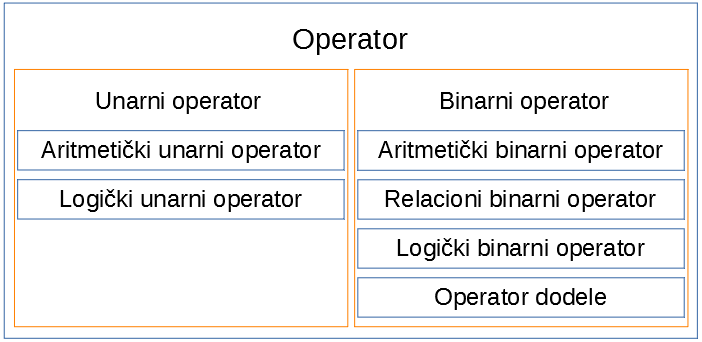
\includegraphics[scale=0.5]{images/operator_nodes.png}
\caption{Podela operatora na osnovu njihove arnosti.}
\label{fig:OperatorNodes}
\end{figure}

Unarni aritmetički operatori su unarni operatori koji figurišu u aritmetičkim izrazima, npr. operator promene znaka, operator bitovske negacije \emph{Bitovski izrazi se mogu posmatrati kao vrsta aritmetičkih izraza}, operatori kastovanja ili inkrementiranja odnosno dekrementiranja. Unarni logički operatori su unarni operatori koji figurišu u logičkim izrazima, npr. operator negacije. Možemo sve ove unarne operatore posmatrati apstraktno ukoliko definišemo unarni operator kao strukturu koja definiše unarnu funckiju koja transformiše svoj argument na osnovu logike konkretnog unarnog operatora. Tip argumenta i povratne vrednosti pomenute funkcije zavisi od tipa unarnog operatora --- aritmetički unarni operatori mogu primiti vrednost bilo kog tipa\footnote{Ne postoji ograničenje na brojevne tipove jer se u nekim jezicima operatori mogu predefinisati tako da rade i za korisnički definisane tipove (engl. \emph{operator overloading}).} i vračaju vrednost proizvoljnog, ne nužno istog tipa; dok unarni logički operatori primaju i vraćaju bulovsku vrednost\footnote{U nekim programskim jezicima postoji implicitna konverzija brojevnih tipova u bulovski tip, što se jednostavno može posmatrati kao poređenje vrednosti po jednakosti sa nulom.}. Koristeći ovaj pristup, nije potrebno praviti novi AST čvor za svaki mogući operator, već je dovoljno da postoji samo jedan čvor koji predstavlja unarni operator. Ovakav pristup odgovara varijanti AST sa regularnošću (videti sliku \ref{fig:ASTVariants}), omogućava opisivanje proizvoljnih operatora i nije vezan za konkretnu programsku paradigmu.

Binarni aritmetički operatori su binarni operatori koji figurišu u aritmetičkim izrazima, npr. operatori koji odgovaraju matematičkim operacijama ali i bitovski binarni operatori. Binarni relacioni operatori su binarni operatori koji figurišu u relacionim izrazima, npr. operatori poretka ($<$, $>$, $\leq$, $\geq$) i poređenja po jednakosti ili različitosti ($=$, $\neq$). Binarni logički operatori su binarni operatori koji figurišu u logičkim izrazima, npr. bulovske operacije ($\wedge$, $\vee$). Slično kao i za unarne operatore, moguće je apstraktno posmatrati sve binarne operatore tako što ih definišemo kao strukturu koja definiše binarnu funkciju koja transformiše argumente na osnovu logike konkretnog binarnog operatora. Tip argumenata i povratne vrednosti te funkcije zavisi od tipa binarnog operatora, kao i u slučaju unarnih operatora --- aritmetički binarni operatori primaju dva argumenta proizvoljnog tipa i vraćaju rezultat proizvoljnog, ne nužno istog tipa; relacioni binarni operatori primaju iste tipove argumenata kao i aritmetički binarni operatori, međutim povratna vrednost mora biti bulovskog tipa; dok logički binarni operatori zahtevaju da argumenti i povratna vrednost budu bulovskog tipa. Pritom, na prvi pogled nije jasno kako se operator dodele može uklopiti u ovaj šablon ali, na osnovu toga da je dodela zapravo sporedni efekat i da se posmatra kao izraz čija je vrednost jednaka vrednosti izraza sa desne strane operatora, može se primeniti isti princip kao i za aritmetičke binarne izraze. Neki programski jezici dozvoljavaju i složene operatore dodele, koji se mogu dekomponovati na više jednostavnijih izraza.
